We now have enough methods to begin approximating both the particle system and the kinetic model. As in previous sections, we first focus on the particle system, before involving the continuum approach. 
\subsection{Space-Homogeneous Particle Model}\label{sec:homparticles}
Recall the homogeneous particle model \eqref{eq:homparticle},
\begin{equation}\tag{\ref{eq:homparticle}}
\dif v^{i,N}_t = G\left(\frac{1}{N}\sum_{j=1}^n v^{j,N}_t\right)\dif t-v^{i,N}_t \dif t + \sqrt{2\sigma} \dif W^i_t.
\end{equation}
Simulating this system is analagous to solving the Ornstein-Uhlenbeck process of Section \ref{sec:particlemethods}. The interaction term is easily calculable using NumPy's \texttt{mean()} function as it is simply the average velocity of all the particles at each time step. The Euler-Maruyama scheme for this system is
\[ v^{i,N}_{n+1} = v^{i,N}_n - v^{i,N}_n\Dt + G\left(\frac{1}{N}\sum_{j=1}^N v^{j,N}_n\right)\Dt+ \sqrt{2\sigma\Dt} Z^i_n. \]
As the system contains interactions, simulating one particle for a long time is no longer sufficient. Multiple particles must be simulated simultaneously. Figure \ref{fig:homparticlemoments} shows how the particle system behaves for a uniform initial distribution with negative mean. The mean velocity is herded towards -1, as predicted in the analysis. The variance behaves similarly, moving towards an average value of 1. Here the mean and variance of velocity is taken at each time step. If instead these statistics were taken across all time up to the point, by setting \texttt{timeavg = True}, the convergence is more clear.
\begin{figure}
    \centering
    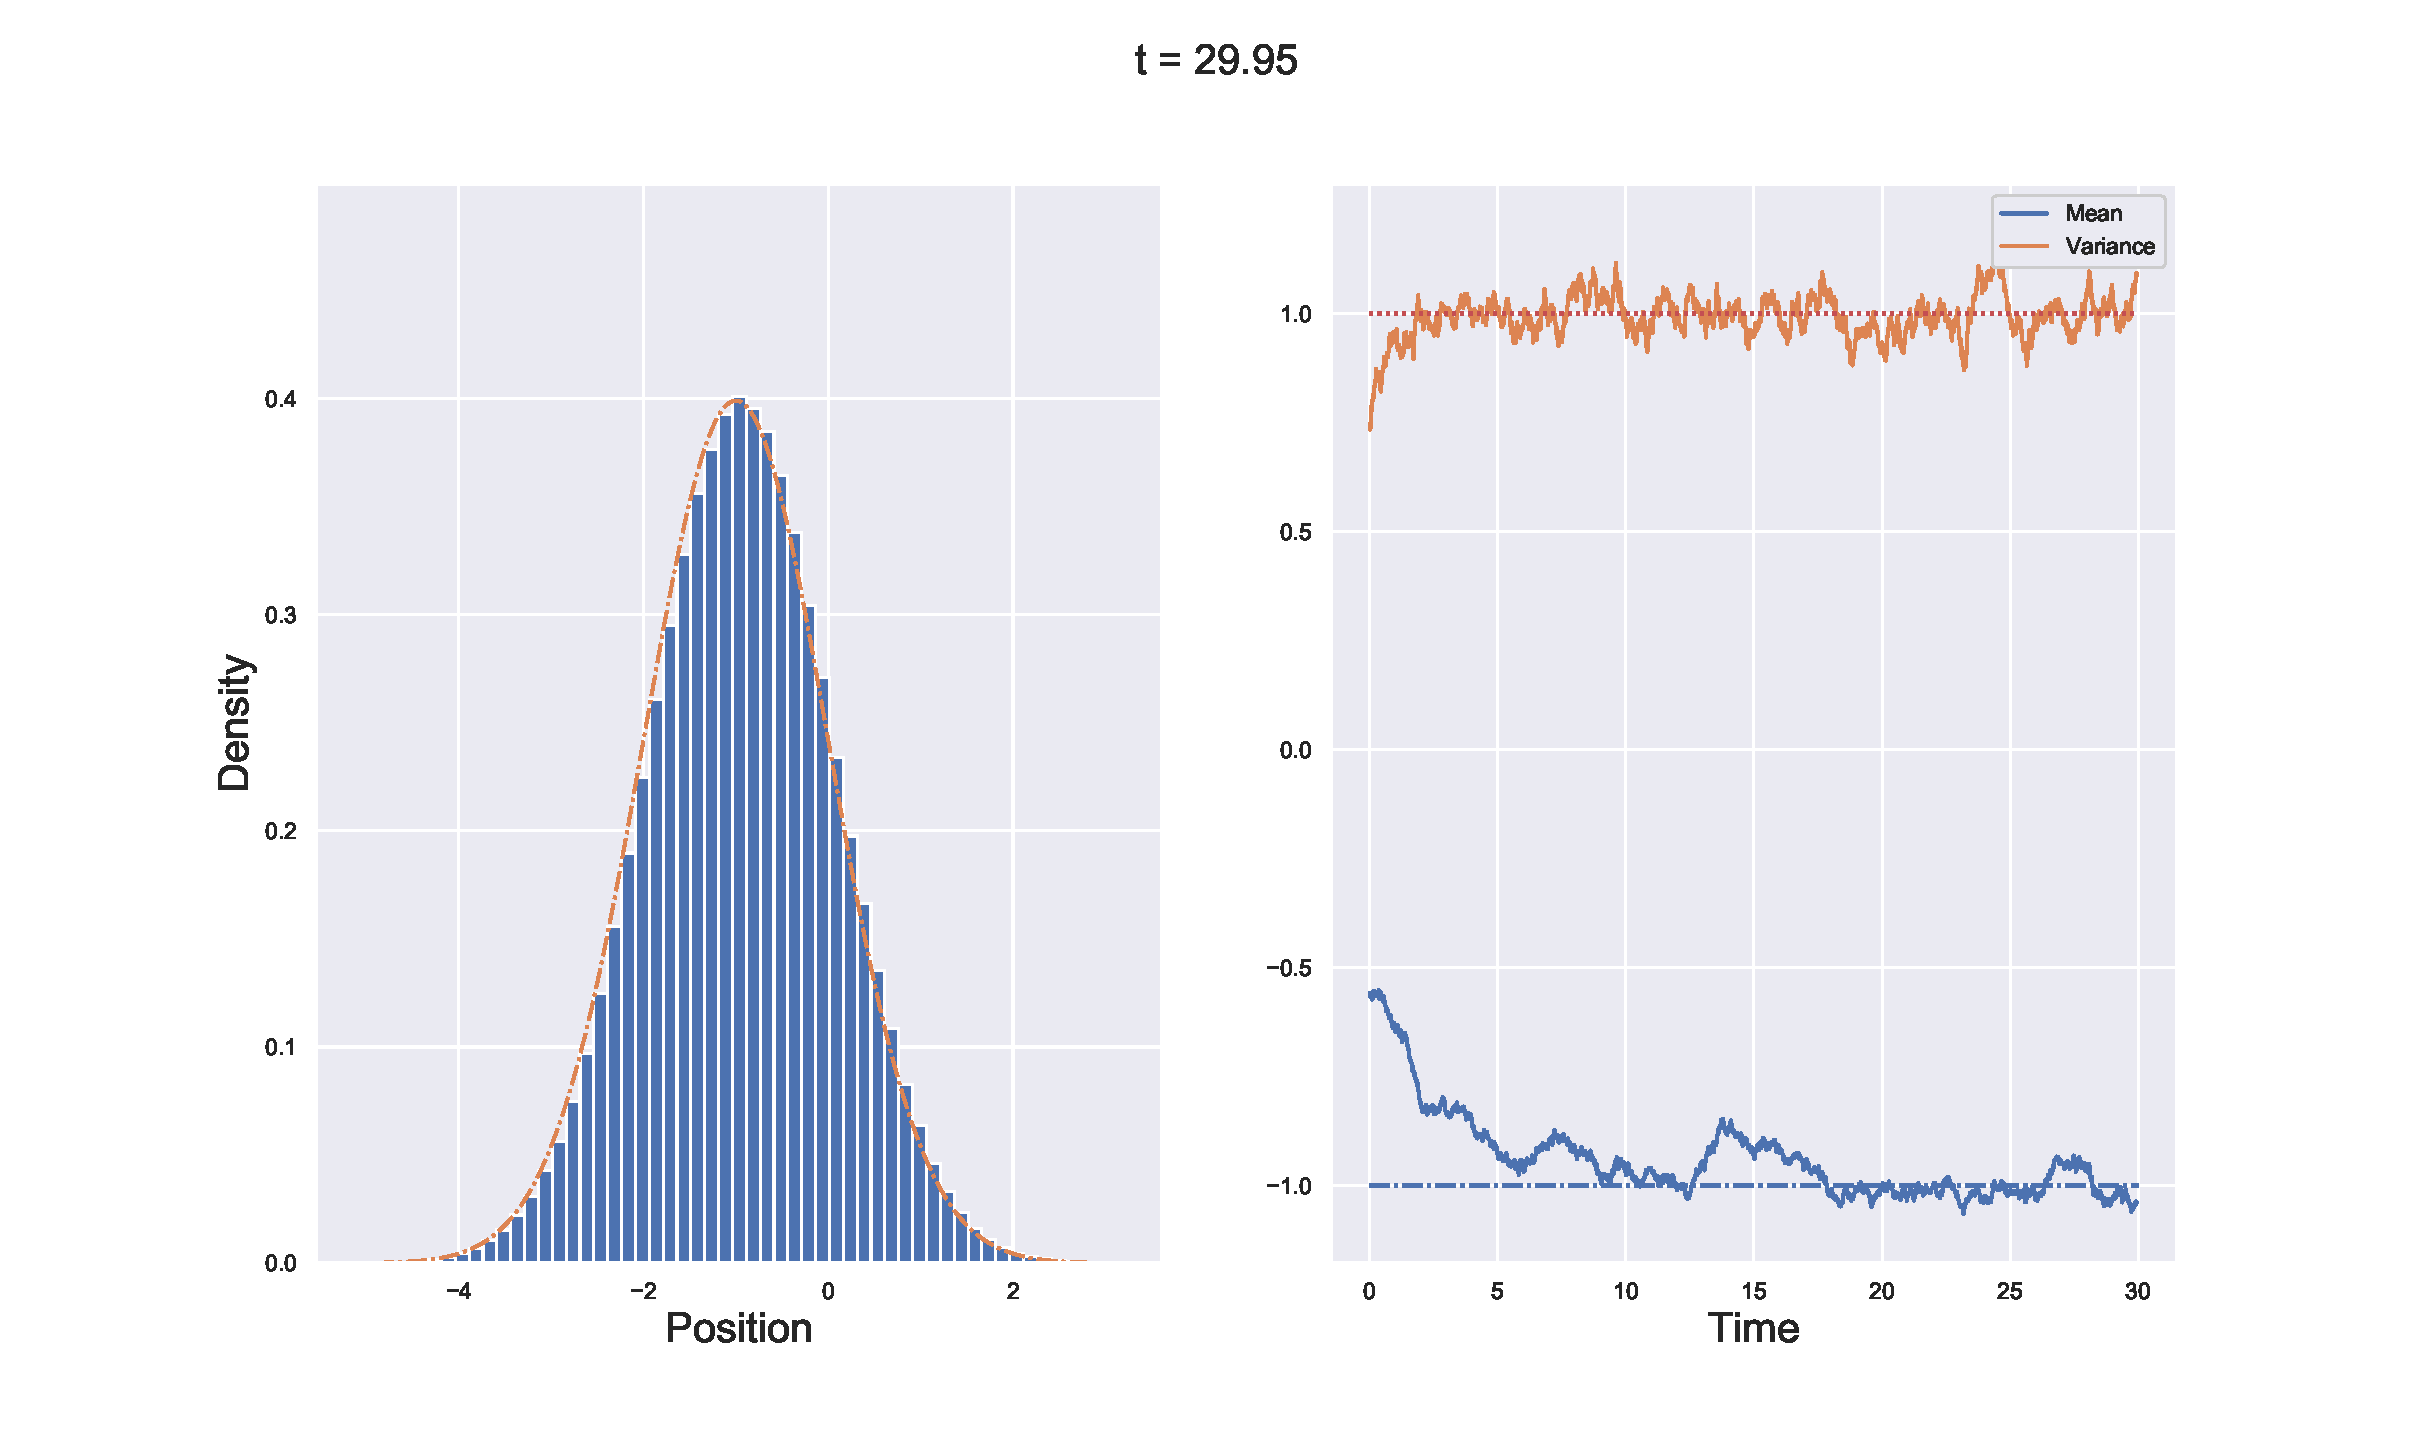
\includegraphics[width=\linewidth]{Figures/homparticles}
    \caption[Homogeneous Particle System]{Histogram of velocities of 1000 particles after 30s with $\sigma = 1$ against the analytic stationary distribution. A time step of $\Dt = 0.01$ was used and the initial data was uniform on $[-2,1]$. The right-hand plot shows the mean and variance moving towards the predicted values and oscillating about them.}
    \label{fig:homparticlemoments}
\end{figure}
We can also plot an animation of the movement of the density of particles over time. Recall from Section \ref{sec:dynamics} that the empirical distribution of the particle system only approximates the true distribution as the number of particles tends to infinity. For any finite number of particles there is only one stationary distribution. When simulating the system, if the number of particles is high enough the probability that enough particles jump across the barrier is very small, and will only be seen if the simulation is ran for an extremely long time. Nevertheless, if the number of particles is low enough, these switches happen often enough to observe, as Figure ++ref+++ shows. 

\begin{figure}
    \centering
    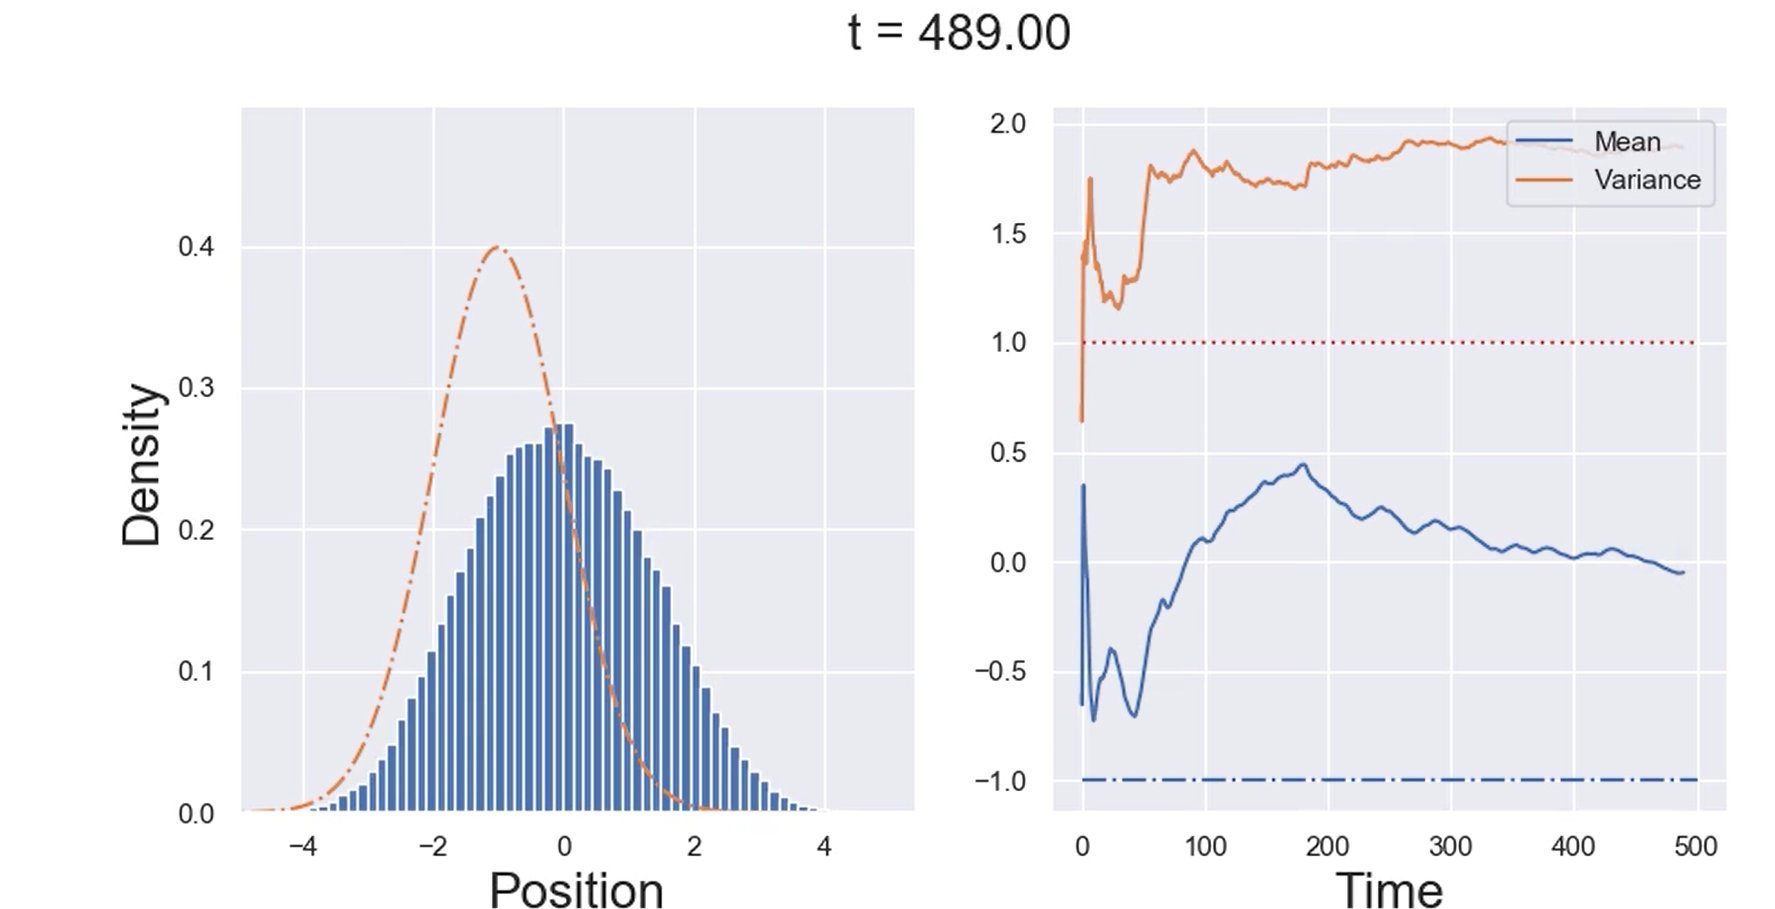
\includegraphics[width=\linewidth]{Figures/switch}
    \caption[Mean Zero Invariant Measure for the Particle System]{}
    \label{fig:switch}
\end{figure}

\subsection{Space-Homogeneous Kinetic Model}\label{sec:homkin}
 Consider the space-homogeneous evolution given by \eqref{eq:spacehomPDE}, that is
    \begin{equation}
    \partial_t f_t(v) = \partial_v vf_t(v) - \partial_v G(\langle w \rangle_{f_t})f_t(v) + \sigma \partial_{vv} f_t(v).
    \end{equation}
    Using the methods developed in the previous section, we are now able to solve this system numerically. As when solving the heat equation, a zero boundary condition shall be enforced. This is valid as we know that the stationary distributions are Gaussian and centred at $-1,0,+1$. The boundary $L$ can then be chosen depending on the the diffusion so that almost no mass is contained beyond the boundary. For example if $\sigma = 1$, the mass contained beyond $L=5$ is of the order $10^{-5}$. 
    
    Simpson's rule will be used as a quick way to approximate the integral within the herding coefficient. To differentiate between the integral and its approximation, we write \(\langle w\rangle_{F^n}\). Below is the scheme when both the herding coefficient and the velocity are positive, using a finite difference scheme with a CN discretisation for the diffusive term and an upwind method for the damping and herding terms.
    \begin{equation*}
    \begin{split}
    \frac{F_j^{n+1} - F_j^n}{\Delta t} = 	-G(\langle w\rangle_{F^n})\left[ \frac{F^n_{j+1} - F^n_{j}}{\Delta v}\right] &+\left[ \frac{v_{j}F^n_{j} - v_{j-1}F^n_{j-1}}{\Delta v}\right]\\ &+ \frac{\sigma}{2}\left[ \frac{F^{n+1}_{j+1} - 2F^{n+1}_j + F^{n+1}_{j-1}}{(\Delta v)^2} + \frac{F^{n}_{j+1} - 2F^{n}_j + F^{n}_{j-1}}{(\Delta v)^2}\right] 	 
    \end{split}
    \end{equation*}
    
    +++Pictures, moments converging, error (in moments too?) in particular, mass loss? -> compare conservative methods i.e. fin vol +++
\subsection{Space-Heterogeneous Particle Model}\label{sec:hetkin}
    +++ phi = 1 still, moving in space. Animations/diagrams showing Leb in space. +++
    